\section{ISO14443}

\begin{frame}
    \frametitle{ISO14443a e NFC}
    \textbf{Cos'è NFC}\\
    Teconologia di comunicazione contactless (short range wireless)
    che permette dispositivi a basso costo\cite{coskun2013survey}

    \pause

    \textbf{Come funziona}
    \begin{itemize}
        \item<1-> Semplificando il tutto, la comunicazione NFC è equivalente a un trasformatore.
        \item<2-> la trasimissione dell'informazione avviene mediante ASK e Load Modulation\cite{instruments2014iso}
    \end{itemize}
\end{frame}
\note{
    La codifica dell'informazione avviene con una variante di  manchester encoding\cite{instruments2014iso}

    Si veda nella prossima slide l'immagine della traccia
}

\begin{frame}
    \begin{figure}
        \centering
        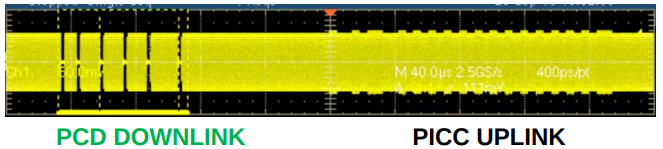
\includegraphics[width=0.95\textwidth]{ISO14443a_COM.png}\cite{instruments2014iso}
        \caption{Traccia della comunicazione tra dispositivo e lettore}
        \label{fig:iso14443a-trace}
    \end{figure}
    Si noti come la frequenza della portante sia notevolmente elevata\pause

    Ciò permette di avere dei dispositivi (TAG) completyamente passivi alimentati dalla portante stessa.
\end{frame}
\note{
    Dall'immagine è possibile osservare come la trasmissione in downlink sia 100\% ASK, dove le tempistiche di bit
    sono notevolmente inferiori ai 13.56MHz della portante.
    Ciò permette al dispositivo di essere completamente passivo e di auto alimentarsi tramite l'effetto trasformatore
    causato dal coupling elettoromagnetico delle due induttanze.
    La trasmissione inversa, dal tag al lettore, di conseguenza non può avvenire allo stesso modo, essendo il tag non in grado di generare
    una portante.
    
    La soluzione è di variare l'impedenza collegata alla spira di ricezione nel tag in modo da utilizzare più corrente.
    Questo causerà una maggiore corrente nel lato trasmettitore che, mediante la resistenza interna di quest'ultimo, causerà una caduta
    di tensione leggibile e interpretabile.
}

\subsection{UUID e anticollisione}
\begin{frame}
    \frametitle{UUID e identificazione multipla di TAG}
    \begin{itemize}
        \item<1-> L'UUID è un codice di identificazione univoco che permette l'identificazione dei tag.
        Un generico tag ISO14443-compilant possiede un UUID di 10byte, ma varie implementazioni permettono di ridurre
        la lunghezza fino a un UUID minimo di 4byte.\cite{nxpmifareuidhandling}
        \item<2-> Mediante il ciclo di identificazione e anticollisione è possibile ottenere la lista di tutti i tag presenti nelle vicinanze del lettore.
        \item<3-> Sarà poi possibile inviare comandi specifici a un solo tag mendiante il processo di selezione
    \end{itemize}
\end{frame}
\note{}

\subsection{Tag MIFARE Classic}
\subsubsection{Struttura della memoria}
\begin{frame}
    \frametitle{MIFARE Classic: Struttura della memoria}
    I tag MIFARE Classic sono tra i più \textbf{semplici} e \textbf{economici}:
    
    Il tag consiste in un piccolo frontend radio e logico che possa gestire la comunicazione
    e in una memoria non volatile dove salvare le configurazioni.\cite{nxpmifareev1datasheet}

    \begin{figure}
        \centering
        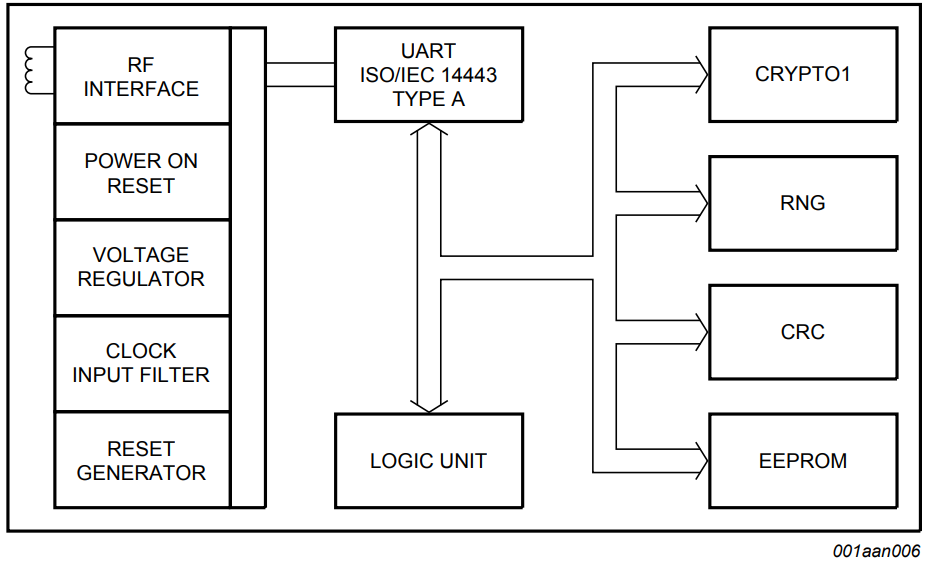
\includegraphics[width=0.45\textwidth]{MIFARE-EV1-INTERNAL_STRUCTURE.png}\cite{nxpmifareev1datasheet}
        \caption{Diagramma dei componenti interni a un chip MIFARE Classic}
        \label{fig:internal-mifare-block-diagram}
    \end{figure}
\end{frame}

\begin{frame}
    La memoria è divisa in \textbf{settori} e \textbf{blocchi}:
    \begin{itemize}
        \item <1-> 16 settori \texttt{[0-15]}
        \item <2-> 4 blocchi per settore \texttt{[0-3]}
        \item <2-> Solo tre blocchi per settore possono includere dati \texttt{[0-2]}
        \item <3-> Il blocco \texttt{0:0} è leggibile senza autenticazione, protetto in scrittura e contiene l'uuid e dati del produttore
        \item <4-> I blocchi \texttt{x:3} contengono le chiavi di scrittura e lettura (\textit{KeyA} e \textit{KeyB}), oltre che gli indicatori di protezione (access bits)
    \end{itemize}
\end{frame}

\subsubsection{Lettura e scrittura}
\begin{frame}
    \frametitle{MIFARE Classic: Lettura e scrittura}
    Prima di effettuare qualunque azione sulla memoria è necessario autenticarsi con la chiave adatta al settore in questione.\pause

    Il processo di autentiocazione è chiamato \textit{``Three pass authentication sequence''}\cite{nxpmifareev1datasheet}
    e sfrutta un cifrario a flusso
\end{frame}
\note{
    Il cifrario a flusso utilizzerà uno stream di dati denominato \(ks_n\) dove n sarà l'n-esima iterazione
}

\subsubsection{Three pass authentication sequence}
\begin{frame}
    \frametitle{Three pass authentication sequence\cite{garcia2008dismantling}}
    {
        \scriptsize
        \begin{columns}[onlytextwidth,T]
            \column{\dimexpr\textwidth-40mm-2mm}
                \begin{itemize}
                    \item <1-> Il tag entra nel campo magnetico del lettore e si accende
                    \item <2-> Protocollo di anticollisione (\textit{Non descritto}) e invio dell'UUID
                    \item <3-> Il lettore effettua una richiesta di autenticazione al blocco richiesto
                    \item <4-> Il tag ritorna un nonce \(n_t\) e lo trasmette in chiaro
                    \item <5-> Il lettore quindi invia il proprio nonce \(n_r\) e la risposta alla challenge \(a_r\)
                            cifrandoli mediante xoring con lo stream proveniente dal cifrario a flusso \(ks_1\) e \(ks_2\)
                    \item <6-> L'autenticazione si conclude con il tag che risponderà alla challenge del reader con \(a_t\) cifrato tramite \(ks_3\)
                \end{itemize}
            \column{40mm}
                \begin{figure}
                    \centering
                    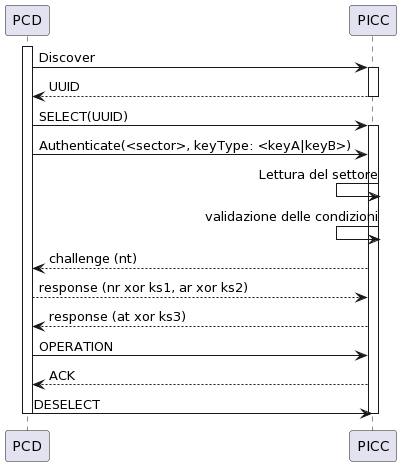
\includegraphics[width=40mm]{AuthSequence.png}
                    \caption{\scriptsize Diagramma di sequenza del processo di autenticazione a un blocco}
                    \label{fig:seq-three-pass-auth}
                \end{figure}
        \end{columns}
    }
\end{frame}
\note{
    sarà possibile evidenziare una vulnerabilità nella generazione di numeri casuali, dipendenti solo dal power on time

    mentre in alcuni tag lo stato del rng è aggiornato solo alla fine di un'autenticazione. ciò comporta che la sequenza di nonce
    del lettore è sempre la stessa
}

\begin{frame}[allowframebreaks]
    \frametitle{Three pass authentication sequence\cite{garcia2008dismantling}}
    In particolare la scelta dei nonce avviene come dalla seguente illustrazione, dove \(key\) è la chiave condivisa
    (ovvero la chiave che il lettore usa per autenticarsi)
    
    Generazione del tag nonce
    \[n_t = nextRandom()\]
    \[send(n_t)\]

    Dopo l'invio, sia il tag che il lettore inizializzano il proprio cifrario a flusso e computano i primi 32bit del \textit{keystream}
    \[ks_1 = cipherInit(key, uid, n_t)\]

    Generazione del reader nonce
    \[n_r = nextRandom()\]

    Invio del reader nonce (cifrato) e dalla risposta alla challeng così computata
    \[a_t = suc^2(n_t)\]
    \[ks_2 = cipher(n_r)\]
    \[send(n_r \oplus ks_1); send(a_t \oplus ks_2)\]
    
    Risposta finale
    \[send(suc^3(n_t) \oplus ks_3)\]
\end{frame}
\note{
    Sia la funzione \(suc(v)\) la successiva iterazione del cifrario di flusso inizializzato cin valore \(v\) 
    
    Il processo di scambio di chiavi viene così descritto:
    \begin{itemize}
        \item il tag sceglie il proprio nonce e lo invia al lettore
        \item entrambe le parti inizializzano il proprio cifrario con una funzione della chiave \(key\), \(n_t\) e l'uid del tag
        \item una volta ottenuto il nonce, il lettore computa i primi 96 bit del keystream \(suc(n_t) = ks_1, suc^2(n_t), suc^3(n_t)\)
        \item il lettore genera \(n_r\) e lo invia al tag cifrandolo con \(ks_1\)
        \item il lettore quindi, dopo aver calcolato \(suc^2(n_t), suc^3(n_t)\) aggiorna il proprio cifrario con il valore \(n_r\), la cui nuova iterazione rappresenterà la seconda chiave, la quale verrà inviata cifrata con la seconda iterazione del cifrario inizializzato precedentemente a fini di verifica
        \item il tag quindi genera le due chiavi necessarie per decifrare i dati, ottenendo così \(n_r\), utilizzato per aggiornare il proprio cifrario e conseguentemente per torvare \(ks_2\) che permetterà di verificare la correttezza di \(suc^2(n_t)\)
        \item per completare l'autenticazione viene quindi inviato \(suc^3(n_t)\) cifrato con \(k_3\) in modo che Il lettore possa validare il tag.
    \end{itemize}
}

